\hbadness=100000
\documentclass[12pt]{article}
\usepackage{hyperref}
\usepackage[left=1in, right=0.5in, top=1in, bottom=1in]{geometry}
\usepackage{tabto}
\usepackage{booktabs}
\usepackage[table]{xcolor}
\usepackage{tabularx}
\usepackage{makecell}
\usepackage{array}
\usepackage{float}
\usepackage{longtable}
\usepackage{amsmath}
\usepackage{amssymb}
\usepackage{lmodern}
\usepackage{graphicx}
\usepackage{multicol}
\usepackage{subcaption}

% ----TITLE PAGE DETAILS----
\title{\bfseries Dataset and Stochastic Instability in Classification Models for Recidivism Risk Prediction}
\author{\bfseries 
 Nikka Angela E. Naputo\\
 CMSC 199.2 Research in Computer Science II\\
 Division of Natural Sciences and Mathematics\\
 University of the Philippines Tacloban College\\
 {\small nenaputo@up.edu.ph}
}
\date{\today}

% ----START THE DOCUMENT----
\begin{document}
\sloppy % Prevent text from extending to other columns

% ----DISPLAY TITLE----
\maketitle 
\newpage 

% ----DISPLAY TABLE OF CONTENTS----
\tableofcontents 
\newpage

% ----1. INTRODUCTION----
\section{Introduction} 
\tabto{2em} Assessing recidivism risk among offenders is important in identifying the risk factors that need to be addressed in order to prevent reoffending~\cite{bonta2007risk, duwe2017out}. Machine learning (ML) models have been developed specifically for recidivism risk prediction (RRP) due to its efficiency, scalability, and complex pattern and relationship detection, enhancing the assessment of recidivism risk in defendants. Such models developed include COMPAS~\cite{northpointe2015practitioner} and MnSTARR~\cite{duwe2014development}, which are statistical ML-based tools. Moreover, other modern ML approaches have been explored to look for models with better predictive accuracy, while also capturing complex, non-linear relationships in recidivism data, such as random forests, support vector machines (SVMs), boosting, and neural networks (NNs)~\cite{duwe2017out}.\\

ML models are used increasingly in actual sentencing decisions. COMPAS, for example, has influenced the sentencing of cases like Loomis in 2013~\cite{loomis2016} and Samsa in 2014~\cite{samsa2014}. As a result, concerns regarding fairness in its use have emerged. In 2016, ProPublica published a report claiming their analysis on the racial fairness of COMPAS found it to be more likely to misclassify black defendants as higher risk and white defendants as lower risk~\cite{propublica2016analysis}. The report garnered criticism for its choice of evaluation metrics, particularly its focus on error rates without considering the differences in recidivism rates across the racial groups. By using alternative metrics such as predictive parity and AUC, the critics found similar levels of predictive performance between Black and White defendants, suggesting that different fairness definitions can lead to differing interpretations of bias~\cite{dieterich2016compas, corbett2017algorithmic, flores2016false}. In addition, developing prediction models that try to address group bias can actually result in inconsistent predictions for the individual-level as offenders with the same attributes could be predicted unfairly due to group membership~\cite{greene2022forks, corbett2017algorithmic}. \\

Predictive inconsistency is a less explored aspect within the literature of machine learning recidivism risk prediction (ML-RRP) as most studies either focus on measuring a model's predictive performance~\cite{duwe2017out, travaini2022machine, tollenaar2013method} or fairness~\cite{tolan2019machine, dressel2018accuracy, ngo2018traditional}. Predictive inconsistency refers to an individual being given varied risk scores due to different, yet equally justifiable technical decisions during model development~\cite{greene2022forks}. This score variability is related to model instability, the formal term used in ML literature referring to multiple models of the same structure producing different predictions on the same individual. A model that is considered unstable undermines its reliability as its predictions cannot be fully trusted~\cite{riley2023stability}, and this becomes particularly critical in risk-sensitive situations where inconsistent predictions could lead to catastrophic outcomes such as harm to humans, major economic loss~\cite{zhang2024reliability}, or in the case of assessing recidivism risk, unfair legal consequences for defendants~\cite{greene2022forks}. \\

The factors that cause model instability include small perturbations in the training data or nondeterministic factors during the model's learning process~\cite{riley2023stability, lopez2022instability}, which this paper distinguishes into two types respectively: dataset instability and stochastic instability.\\

Though prior studies on ML-RRP often examine these models' performance and fairness, comparatively little attention has been given to exploring their instability as existing literature either do broad conceptual analyses on the factors that cause predictive inconsistency~\cite{greene2022forks}, or have only studied the instability of actuarial tools used in RRP~\cite{helmus2015stability}, not models. Moreover, as these models continue to be used for sentencing decisions, their predictions carry profound and potentially detrimental impact on a defendant's legal status and freedom~\cite{van2022predicting}. \\

Therefore, examining the instability of ML models in RRP is essential, as it addresses major concerns regarding a model's prediction reliability on the individual level, and the risk that inconsistent predictions could lead to, such as unfair legal outcomes and sentencing decisions, while filling the clear gap of lacking instability studies within the current ML-RRP literature.\\
\newpage

% ----1.1 BACKGROUND OF THE STUDY
\subsection{Background of the Study}
\subsubsection{Recidivism Risk Assessment} 
\tabto{2em} Recidivism risk assessment is the use of statistical or algorithmic tools to predict the likelihood an individual will re-engage in criminal behavior after being punished or released~\cite{ozkan2017predicting}. These tools help judges, administrators, and correctional officers make informed decisions about a defendant with regards to their pretrial detention, sentencing, and inmate placement~\cite{corbett2017algorithmic}.\\

% Talks about the four generations of risk assessment tools
\textbf{There are four generations of risk assessment tools:}
\begin{enumerate}
 \item \textbf{First Generation (Pre-1950s):} Offender risk assessment was primarily based on subjective, professional judgements made by correctional staff~\cite{duwe2017out,ozkan2017predicting}. However, these assessments were often vulnerable to individual bias and inconsistency.
 \item \textbf{Second Generation (Late 1920s-1970s):} This era saw the introduction of objective actuarial methods which focused on static factors such as criminal history~\cite{duwe2017out}. 
 \item \textbf{Third Generation:} Recognizing the limitations of the second generation risk assessment tools, these tools began incorporating dynamic risk factors (criminogenic needs), which are factors that change over time and serve as targets for intervention, such as employment status or substance abuse, alongside static factors~\cite{duwe2017out}. 
 \item \textbf{Fourth Generation:} These are the modern recidivism risk assessment tools that continuously assess defendants throughout their involvement in the justice system, tracking changes over time and considering both risk and protective factors to guide the decisions of criminal justice practitioners~\cite{duwe2017out}.
\end{enumerate}

The evolution of these tools reflects a shift toward more data-driven and dynamic approaches to risk assessment, which has paved the way for the integration of ML approaches in RRP.\@

\subsubsection{Machine Learning}
\tabto{2em} Machine Learning (ML) is a branch of artificial intelligence that focuses on algorithms capable of learning patterns from data without explicit programming~\cite{duwe2017out}. ML models are commonly categorized into two types based on their learning approach: Supervised and Unsupervised Learning Models.\\

Supervised learning models are trained using labeled data with known outcomes and are used to generate predictions. Supervised learning has been applied across multiple domains such as healthcare, finance, marketing, engineering, and criminal justice due to its ability to model complex relationships and efficiently process large volumes of data~\cite{duwe2017out,ozkan2017predicting}. In the context of criminal justice, supervised ML models are used in risk assessment to support decision-making processes, such as prioritizing limited resources toward higher-risk defendants and informing interventions for those assessed as lower risk.\\

In contrast, unsupervised learning models are trained without a labeled outcome measure. They describe associations and patterns among input variables rather than predicting a target~\cite{duwe2017out}. In a recidivism study, Cavus et al. combined k-means clustering with neural-network prediction: clustering identified groups of offenders with similar profiles, and group-specific neural networks estimated recidivism risk within each group~\cite{cavus2025transparent}.\\

\subsubsection{Machine Learning For Recidivism Risk Prediction}
\tabto{2em} Since the 1990s, ML-based recidivism risk assessment tools have been developed to predict the likelihood of reoffending. Examples include the Correctional Offender Management Profiling for Alternative Sanctions (COMPAS), developed by Northpointe in 1998 using statistical and ML methods~\cite{northpointe2015practitioner}, and the Minnesota Screening Tool Assessing Recidivism Risk (MnSTARR), developed by Duwe in 2014 which utilizes multiple logistic regression modeling due to its interpretability that allows researchers to discern exactly how much each variable contributes to a final prediction~\cite{duwe2014development}.\\

These tools are used to support criminal justice decisions such as sentencing, pretrial detention, and offender supervision. In some cases, judicial decisions have been influenced by the outputs of these models. For example, in the case of Eric Loomis in 2013, the COMPAS assessment included in his Pre-Sentence Investigation (PSI) labeled him as “high risk” for recidivism, which was considered during sentencing~\cite{loomis2016}. Similarly, in the case of Jordan Samsa in 2014, the court considered components of the COMPAS report, such as criminogenic needs, in determining sentencing outcomes~\cite{samsa2014,liu2019beyond}.\\

Beyond existing risk assessment tools, general supervised ML models have also been explored for RRP such as logistic regression, random forests, gradient-boosted trees, and support vector machines~\cite{duwe2017out,ozkan2017predicting,ngo2018traditional}.

\begin{enumerate}
 \item \textbf{Logistic Regression} \\
  \tabto{2em} Logistic Regression (LR) is a statistical classification model that estimates the probability of an outcome from a linear combination of input features. It is widely used as a baseline in recidivism risk prediction because its coefficients offer a relatively direct way to interpret how features relate to the outcome~\cite{travaini2022machine}. Logistic regression was also used in developing the Minnesota Screening Tool Assessing Recidivism Risk (MnSTARR)~\cite{duwe2014development}.\\

  For a binary outcome, the model represents the log-odds of the positive outcome as a linear function of the features:
  \[
  \log\!\left(\frac{P(Y_i=1\mid\mathbf{x}_i)}{1-P(Y_i=1\mid\mathbf{x}_i)}\right)
  = b_0+\sum_{j=1}^{p}b_jx_{ij}.
  \]
  Applying the inverse logit, or sigmoid, function gives the positive-class probability:
  \[
  \hat{p}_i=P(Y_i=1\mid\mathbf{x}_i)
  =\frac{1}{1+\exp\!\left[-\left(b_0+\sum_{j=1}^{p}b_jx_{ij}\right)\right]}.
  \]
  Here, $\mathbf{x}_i$ is the feature vector for instance $i$, $x_{ij}$ is feature $j$, $b_j$ is its coefficient, and $b_0$ is the intercept. A coefficient $b_j$ gives the change in log-odds associated with a one-unit increase in feature $j$, holding other features fixed; equivalently, the odds are multiplied by $e^{b_j}$. The resulting probability can be assigned to a class using a decision threshold.\\

 \item \textbf{Random Forest}\\
  \tabto{2em} Random Forest (RF) is an ensemble of decision trees. It builds trees using bootstrap samples of the training data and considers randomly selected subsets of features when splitting nodes. These sources of randomness make the trees less alike; combining their predictions can reduce the variance of an individual tree~\cite{kovalchuk2023prediction}. Random forests have been applied to recidivism risk prediction and are among the commonly examined models in this literature~\cite{travaini2022machine}.\\

  For classification, the forest can average the class probabilities estimated by its $B$ trees and select the class with the largest average:
  \[
  \hat{P}(Y_i=k\mid\mathbf{x}_i)=\frac{1}{B}\sum_{b=1}^{B}\hat{P}_b(Y_i=k\mid\mathbf{x}_i),
  \qquad
  \hat{y}_i=\underset{k\in\{0,1\}}{\arg\max}\;\hat{P}(Y_i=k\mid\mathbf{x}_i).
  \]
  Here, $\hat{P}_b(Y_i=k\mid\mathbf{x}_i)$ is the probability assigned to class $k$ by tree $b$. This probability-averaging description distinguishes the forest's prediction from majority voting over hard class labels.\\

 \item \textbf{XGBoost}\\
  \tabto{2em} XGBoost is a gradient-boosted decision tree method. It builds an additive ensemble sequentially: each new tree is chosen to improve the objective given the predictions of the trees already added. This is often described informally as correcting previous errors; more generally, the improvement is guided by gradient information from the chosen loss function. XGBoost has been studied for recidivism prediction, including work using it to forecast recidivism and as part of a winning solution to the National Institute of Justice forecasting challenge~\cite{won2019recidivism,rajendran2021predicting,han2022xgboost}.\\
  
  For binary classification, the trees produce an additive raw score, which is transformed into a probability by the sigmoid function:
  \[
  F(\mathbf{x}_i)=b_0+\sum_{t=1}^{T}f_t(\mathbf{x}_i),
  \qquad
  \hat{p}_i=P(Y_i=1\mid\mathbf{x}_i)=\frac{1}{1+e^{-F(\mathbf{x}_i)}}.
  \]
  Here, $f_t$ is the score produced by tree $t$, $T$ is the number of trees, and $b_0$ is an initial score. The training objective combines prediction loss with a penalty on tree complexity:
  \[
  \mathcal{L}=\sum_{i=1}^{n}\ell(y_i,\hat{p}_i)+\sum_{t=1}^{T}\Omega(f_t),
  \]
  where $\ell$ is the binary logistic loss, $\ell(y_i,\hat{p}_i)=-y_i\log\hat{p}_i-(1-y_i)\log(1-\hat{p}_i)$, and $\Omega$ penalizes tree complexity. A common tree penalty is
  \[
  \Omega(f_t)=\gamma J_t+\frac{\lambda}{2}\sum_{j=1}^{J_t}w_{tj}^{2},
  \]
  where $J_t$ is the number of leaves in tree $t$, $w_{tj}$ is the score assigned to leaf $j$, and $\gamma$ and $\lambda$ control the penalties. Each new tree is added to reduce this regularized objective, so the final score is an additive sum of tree outputs rather than a vote among trees.\\

 \item \textbf{Linear Support Vector Machines (SVMs)}\\
  \tabto{2em} Support Vector Machines (SVMs) are classification models that seek a decision boundary with a large margin between classes. SVMs have been examined in recidivism risk prediction alongside other supervised learning methods~\cite{duwe2017out,tolan2019machine,ozkan2017predicting}. A linear SVM uses a linear boundary in the feature space; nonlinear SVMs can represent more complex boundaries through other formulations~\cite{tollenaar2013method,duwe2017out,dressel2018accuracy}. Only linear SVMs are discussed here.\\

  With labels encoded as $y_i\in\{-1,+1\}$, the linear SVM decision function and predicted class are
  \[
  f(\mathbf{x}_i)=\mathbf{w}^{\mathsf T}\mathbf{x}_i+b,
  \qquad
  \hat{y}_i=\operatorname{sign}\!\left(f(\mathbf{x}_i)\right),
  \]
  where $\mathbf{w}$ determines the boundary's orientation and $b$ its offset. A common soft-margin formulation is
  \[
  \min_{\mathbf{w},b,\boldsymbol{\xi}}\quad
  \frac{1}{2}\|\mathbf{w}\|_2^2+C\sum_{i=1}^{n}\xi_i
  \quad\text{subject to}\quad
  y_i(\mathbf{w}^{\mathsf T}\mathbf{x}_i+b)\geq 1-\xi_i,\quad \xi_i\geq0.
  \]
  The slack variables $\xi_i$ allow points to fall within the margin or be misclassified; $C$ controls the trade-off between a wide margin and violations. An SVM's decision function is a signed score rather than a probability, so probability estimates require a separate calibration procedure.\\

 \item \textbf{Multilayer Perceptron (MLP)}\\
  \tabto{2em} A Multilayer Perceptron (MLP) is a feedforward neural network in which each layer transforms the outputs of the previous layer. Its learned weights and nonlinear activation functions allow it to represent nonlinear relationships among input features. Neural networks, including MLPs, have been evaluated in recidivism risk prediction alongside other supervised learning methods~\cite{duwe2017out,travaini2022machine}.\\

  The transformation at hidden layer $\ell$ is
  \[
  \mathbf{h}_i^{(0)}=\mathbf{x}_i,
  \qquad
  \mathbf{h}_i^{(\ell)}=\phi^{(\ell)}\!\left(W^{(\ell)}\mathbf{h}_i^{(\ell-1)}+\mathbf{b}^{(\ell)}\right),
  \quad \ell=1,\ldots,L,
  \]
  where $\mathbf{x}_i$ is the input vector, $W^{(\ell)}$ and $\mathbf{b}^{(\ell)}$ are the weights and biases for layer $\ell$, and $\phi^{(\ell)}$ is its activation function. For binary classification, the output layer maps the final hidden representation to a probability:
  \[
  \hat{p}_i=P(Y_i=1\mid\mathbf{x}_i)
  =\sigma\!\left(\mathbf{w}_{o}^{\mathsf T}\mathbf{h}_i^{(L)}+b_o\right),
  \qquad \sigma(z)=\frac{1}{1+e^{-z}}.
  \]
  The model's weights and biases are learned by minimizing a prediction loss, commonly binary cross-entropy, using gradients computed through backpropagation. A decision threshold can then convert the predicted probability into a class label. Compared with LR's single linear predictor, hidden layers with nonlinear activations can represent more complex feature relationships, though their learned parameters are less directly interpretable.\\
\end{enumerate}

\subsubsection{Concerns in Machine Learning-Based Risk Assessment}
\tabto{2em} With the increasing use of ML models in criminal justice decision-making, several concerns have been raised regarding their application.\\

One major concern involves fairness. In 2016, ProPublica published an analysis of the COMPAS risk assessment tool, reporting that it was more likely to misclassify Black defendants as higher risk and White defendants as lower risk~\cite{propublica2016analysis}. The report garnered criticism from both Northpointe and other researchers for its choice of evaluation metrics, particularly its focus on error rates without considering the differences in recidivism rates across the racial groups. By using alternative metrics such as predictive parity and AUC, the critics found similar levels of predictive performance between Black and White defendants, suggesting that different fairness definitions can lead to differing interpretations of bias~\cite{dieterich2016compas, corbett2017algorithmic, flores2016false}. Fairness-constrained decision rules may apply group-specific thresholds to risk scores, allowing defendants with the same score to receive different decisions based on group membership~\cite{corbett2017algorithmic}.

Predictive inconsistency is a less extensively explored concern within the ML-RRP literature as most studies focus on measuring predictive performance~\cite{duwe2017out, travaini2022machine, tollenaar2013method} and fairness~\cite{ tolan2019machine, dressel2018accuracy,ngo2018traditional}. Predictive inconsistency refers to the variability in risk scores assigned to the same individual due to different, yet equally justifiable, technical decisions made during model development~\cite{greene2022forks}. This variability is closely related to model instability, where models with the same structure may produce different predictions for the same individual~\cite{greene2022forks}.

\subsubsection{Instability in Machine Learning}
\tabto{2em} Instability in ML refers to the sensitivity of a model's predictions to small changes in its training conditions~\cite{sun2015stability}. The most commonly discussed form of instability is dataset instability, which refers to the variability in a model's predictions due to small perturbations in the training data, such as resampling from the original dataset, removing individual data points, or introducing noisy data~\cite{riley2023stability,hardt2016train}. Another form of instability is stochastic instability, which arises from nondeterministic factors in the training process, such as random initialization and data ordering during learning~\cite{lopez2022instability}. This randomness, typically controlled through the model's random seed, can cause models to produce different predictions across runs.\\

An unstable model undermines reliability, as its predictions may not be consistent or dependable~\cite{riley2023stability}. This becomes particularly critical in risk-sensitive contexts, where inconsistent predictions may lead to harmful or high-cost outcomes~\cite{zhang2024reliability}. In the domain of criminal justice, the use of unstable models for recidivism risk assessment could result in unfair legal outcomes for defendants~\cite{greene2022forks}.

% ----2. RELATED WORKS----

\section{Related Works}
\tabto{2em} A large volume of work in RRP focuses on evaluating the overall predictive performance of different ML approaches, particularly comparing traditional models with modern ones.\\

Duwe and Kim~\cite{duwe2017out} compared 12 supervised learning algorithms, including logistic regression, random forests, support vector machines, neural networks, and boosting techniques, using a large dataset of offenders released from prison. Their evaluation considered multiple dimensions of predictive validity, such as discrimination, calibration, and accuracy, across different scenarios varying in sample size, base rates, and predictor sets. While some ML methods, particularly boosting-based approaches like LogitBoost, achieved slightly higher predictive performance, the overall differences between models were relatively modest. This is similar to the findings of Travaini et al.~\cite{travaini2022machine}, who provided a comprehensive overview of the growing application of ML techniques in RRP.\@ Their study analyzed multiple empirical works employing various datasets and models, including logistic regression, random forest, neural networks, and ensemble approaches, to evaluate predictive performance using metrics such as accuracy and AUC.\@ Their findings indicate that across studies, most ML models achieve relatively strong predictive performance, with average results suggesting reliable classification of recidivism outcomes but that no single model consistently outperforms others.\\

These studies highlight that although more complex ML models are capable of capturing nonlinearities and high-dimensional interactions, their practical advantage in RRP is often limited, with simpler statistical models continuing to provide competitive performance. Moreover, model predictive performance is also context-dependent, meaning it is influenced by factors besides model structure.\\

Other than predictive performance, researchers have also increasingly examined the fairness and ethical implications of using ML models in criminal justice settings.\\

Tolan et al.~\cite{tolan2019machine} evaluated the predictive performance and fairness of ML models in comparison to structured human risk assessments within a juvenile justice context. Using a dataset of Catalonian youth offenders, they compared multiple ML models against the SAVRY framework, a structured professional judgement tool used by experts. Their results showed that ML models achieved slightly higher predictive performance, with AUC values improving when more features were included. At the same time, the models exhibited disparities across demographic groups, particularly with respect to sex and nationality. For instance, certain groups such as foreign nationals were more likely to be incorrectly classified as high risk, even when they did not recidivate. The study shows that higher predictive performance did not ensure fairness in this setting: it identifies disparities alongside performance gains but does not establish that optimizing for accuracy caused those disparities. This aligns with an earlier investigation by ProPublica~\cite{propublica2016analysis}, where they raised concerns regarding racial bias in COMPAS by conducting an empirical analysis of over 10,000 defendants from Broward County, Florida. Their study compared COMPAS risk predictions with actual recidivism outcomes over a two-year period and found that, while overall accuracy was moderate (around 61\%), the errors were distributed unevenly across racial groups. Specifically, Black defendants were significantly more likely to be falsely classified as high risk despite not reoffending, while White defendants were more likely to be incorrectly labeled as low risk despite recidivating. Even after controlling for factors such as prior offenses, age, and gender, Black defendants were still more likely to receive higher risk scores. These findings suggest that algorithmic predictions may systematically disadvantage certain demographic groups, raising critical concerns about fairness in risk assessment tools.\\ 

The ProPublica investigation ultimately sparked widespread debate on the ethical implications of using ML in criminal justice decision-making. Representing Northpointe, Dieterich et al.~\cite{dieterich2016compas} reanalyzed the same Broward County dataset and challenged the claim of racial bias. Their study argued that ProPublica relied on incorrect classification statistics, particularly focusing on false positive and false negative rates without accounting for differing base rates of recidivism across racial groups. By instead evaluating metrics such as predictive parity and AUC, they found that COMPAS exhibited similar predictive accuracy for Black and White defendants, indicating what they termed ``accuracy equity''. Their results showed that differences in error rates could arise naturally from underlying differences in group distributions, rather than from algorithmic bias. Consequently, they concluded that fairness assessments depend heavily on the choice of evaluation metric, and that alternative definitions can lead to different interpretations of bias. In addition, Flores et al.~\cite{flores2016false} provided a critical response to the ProPublica analysis, arguing that its conclusions were based on methodological and statistical shortcomings. They emphasized that ProPublica did not follow established standards for testing predictive bias and instead relied on inappropriate comparisons of group-level error rates. Using alternative analytical approaches, including AUC comparisons and regression-based methods, they found no consistent evidence of racial bias in the predictive performance of COMPAS.\@ Their findings reinforce the argument that conclusions about bias are highly sensitive to the evaluation framework and statistical methodology employed.\\

Studies have also explored how fairness constraints can result in different decisions for individuals. Corbett-Davies et al.~\cite{corbett2017algorithmic} investigated the trade-offs between maximizing public safety and satisfying formal definitions of fairness. By formulating fairness as a constrained optimization problem, they showed that satisfying statistical parity, conditional statistical parity, or predictive equality can require group-specific risk thresholds, whereas the unconstrained safety-maximizing rule uses a single threshold for all individuals. Under the statistical parity constraint in their Broward County analysis, they estimated that 17\% of those detained would be low risk and that violent recidivism among released defendants would increase by 9\% relative to the safety-maximizing rule; the other fairness constraints produced different estimates. Because group-specific thresholds can assign different decisions to the same risk estimate, a defendant's race may affect whether that person is detained under a fairness-constrained rule. 

Predictive inconsistency is a less explored aspect within the ML-RRP literature despite multiple studies focusing on measuring predictive performance and fairness. Greene et al.~\cite{greene2022forks} defines predictive inconsistency as the phenomenon where equally justifiable modeling decisions can produce different predicted risk scores for the same individual. This perspective highlights that variability in predictions does not solely arise from model randomness, but also from technical choices made throughout the model pipeline, including data selection, preprocessing, and model structure. Similar to Corbette-Davies et al., Greene et al.\ mentions fairness selection as one of these ``forking paths'' as there is no single definition to fairness. In high-stakes domains such as criminal justice, such inconsistencies raise concerns regarding the reliability and legitimacy of algorithmic risk assessment tools.\\

The variability described by Greene et al.\ can be understood in relation to model instability, the formal term used within ML literature that refers to the variability of predictions that are caused by small perturbations in the training data or stochastic elements in the training process. This connects to algorithmic stability explored by Sun~\cite{sun2015stability} where it is defined as the consistency of a model's predictions under small perturbations in the training data. Through both theoretical analysis and empirical experiments, Sun demonstrated that models with similar predictive accuracy can exhibit significantly different levels of stability, highlighting that accuracy alone is insufficient to evaluate model behavior. The findings emphasize that unstable models may undermine reproducibility and user trust, especially in applications where consistent predictions are critical. \\

% dataset and stochastic instability
Model instability has been explored in other domains, such as in healthcare. Riley and Collins~\cite{riley2023stability} proposed a comprehensive framework for evaluating instability in clinical prediction models across multiple levels. Their approach uses bootstrap resampling to repeatedly reconstruct models from the same dataset, allowing the assessment of how predictions vary under small perturbations in the training data. The study defines several levels of instability, including variability in overall estimated risk, changes in the distribution of predictions, subgroup-level instability, and instability at the individual prediction level. To quantify these effects, they introduced measures such as the mean absolute prediction error (MAPE), which captures the deviation between predictions from bootstrap models and the original model. Their findings demonstrate that even small changes in the dataset can lead to noticeable variability in model predictions, particularly in small sample sizes or high-dimensional settings, despite stable overall performance metrics. This variability was especially evident at the individual level, where predictions for the same individual could differ significantly across models. These results highlight how small changes in the dataset can influence model instability in clinical settings, potentially affecting clinical decision-making, and emphasize the need to evaluate models beyond traditional performance metrics. \\

Beyond dataset-related sources of variability, instability can also arise from the stochastic nature of model training itself. Lopez-Martinez et al.~\cite{lopez2022instability} further examined instability in clinical risk prediction models, particularly focusing on deep learning approaches used for risk stratification. Using electronic health record (EHR) data, they conducted repeated training runs of identical models with different random seeds and showed that model predictions can vary significantly at the individual level despite similar aggregate performance metrics such as ROC-AUC and PR-AUC.\@ To quantify this variability, they introduced metrics such as the Top-K Jaccard similarity, which measures the consistency of high-risk individuals selected across model runs, and rank correlation measures to assess stability in prediction ordering. Their results demonstrate that deep learning models tend to exhibit greater instability compared to simpler models such as logistic regression, particularly in scenarios involving resource allocation where only top-risk individuals are considered. Additionally, the study showed that instability can lead to inconsistent decision-making and variability in subgroup representation, raising concerns about fairness and reliability in deployment settings.\\

% model reliability
While stability focuses on variability in predictions, a closely related concern is the reliability of individual predictions. Zhang and Bose~\cite{zhang2024reliability} introduced Model Reliability for Individual Prediction (MRIP), which estimates the probability that a model's prediction error for an individual falls within a tolerance when considering nearby inputs. When outcomes for synthetic perturbations are unavailable, their method estimates this probability using observed neighboring examples. Their study develops and evaluates MRIP for numerical prediction; applying the indicator to binary classification, as in this thesis, is an adaptation. MRIP provides a local reliability measure that complements aggregate performance metrics, which may not reveal large errors for specific individuals. Similarly, Biddle~\cite{biddle2022predicting} examined the epistemic risks inherent in ML systems, particularly in the context of RRP.\@ Drawing from philosophy of science, the study argues that predictive models are inherently value-laden, as their design involves trade-offs between different types of errors and uncertainties that can disproportionately impact individuals. In high-stakes domains such as criminal justice, these epistemic risks translate into real-world consequences, where unreliable predictions may lead to unjust or harmful decisions. Together, these works highlight that beyond accuracy and fairness, understanding and quantifying the reliability of individual predictions is crucial for the responsible deployment of ML systems.\\

Despite the growing body of work focusing on predictive performance and fairness, there are still limited empirical studies on instability in ML-based RRP literature. One notable study by Helmus and Thornton~\cite{helmus2015stability} examined the stability of actuarial risk assessment tools by analyzing the predictive accuracy of individual items across multiple samples. Their findings showed that while most items were generally predictive, roughly half exhibited significant cross-sample variability in predictive accuracy, often in the magnitude rather than the direction of their predictive association. This indicates variation in how strongly individual items predicted sexual recidivism across samples; it does not directly establish instability in individuals' risk estimates. However, this line of work focuses on traditional actuarial instruments such as Static-99R and Static-2002R, and does not extend to modern ML-based approaches.\\

Overall, the existing literature demonstrates that while substantial progress has been made in evaluating RRP models in terms of predictive performance and fairness, these perspectives alone are insufficient to fully understand model behavior. Studies on model instability highlight that models with similar aggregate performance can produce significantly different predictions at the individual level, influenced by factors such as data perturbations and stochastic training processes. Furthermore, research in other domains, particularly healthcare, shows that such instability is not merely theoretical but can have practical consequences for decision-making, reinforcing the importance of evaluating prediction variability. Despite these insights, the application of instability and reliability analysis to ML-based RRP remains limited, with existing work focusing on traditional actuarial tools. This gap motivates the present study, which aims to empirically analyze the instability of ML models in RRP, considering both dataset and stochastic sources of variability, and to assess how such instability affects individual-level predictions while also evaluating model predictive performance, fairness, and reliability.

% ----3. STATEMENT OF THE PROBLEM----

\section{Statement of the Problem} 
\tabto{2em} ML models are increasingly used in RRP to support decision-making processes within the criminal justice system, particularly in assessing a defendant's risk of reoffending. While numerous studies have focused on evaluating the predictive performance and fairness of these models, comparatively limited attention has been given to their stability. Model instability, which refers to the variability of predictions under small changes in training data or stochastic processes, may result in different predictions for the same individual across model runs or different modeling conditions. This phenomenon is closely related to the broad concept of predictive inconsistency, where equally valid modeling choices can yield divergent outcomes. In high-stakes domains such as criminal justice, such inconsistencies raise concerns regarding the reliability and trustworthiness of algorithmic risk assessments, as they may influence decisions that affect a defendant's personal freedom and legal status.\\

Although prior research has explored instability in traditional actuarial risk assessment tools or conducted a conceptual analysis on the forking paths that cause predictive inconsistency, there remains a lack of empirical studies examining instability in ML-based RRP models. In particular, it is unclear to what extent these models exhibit instability when subjected to variations in training data and stochastic factors during training. Furthermore, the manner in which instability manifests across different evaluation dimensions, such as predicted scores, ranking of individuals, classification outcomes, contextualized with predictive performance, fairness, and reliability, remains underexplored. It is also not well understood how instability varies across different model types or which input features contribute most to unstable predictions.\\

This study addresses these gaps by empirically analyzing the instability of classification models used in RRP.\@ Specifically, it examines how model predictions vary under perturbations in the training data and stochastic training conditions, evaluates instability alongside predictive performance, fairness, and reliability metrics, and identifies key factors that contribute to variability in predictions.

\section{Objectives of the Study} 
\subsection{General Objective} Evaluate dataset and stochastic instability  in classification models for recidivism risk prediction alongside its performance, fairness, and reliability, and feature contribution.
\subsection{Specific Objectives}
\begin{enumerate}
 \item Assess dataset instability by retraining models on bootstrapped, K-fold training samples.
 \item Assess stochastic instability by retraining models with different random seeds across K-fold training partitions.
 \item Evaluate instability, performance, fairness, reliability, and feature contributions using validation and official test predictions.
 \item Analyze how instability, model structure, and feature contributions relate to predictive inconsistency.
\end{enumerate}

\section{Significance of the Study}
\tabto{2em} This study contributes to the growing body of research on ML-RRP by addressing a relatively underexplored aspect: model instability. While prior studies have largely focused on evaluating model predictive performance and fairness, this research focuses on model instability, which is closely related to both predictive inconsistency and reliability. Studying it highly significant within a high\-stakes domain such as criminal justice where model outputs may influence legal decisions and defendant outcomes.\\

By empirically analyzing both dataset instability and stochastic instability across multiple classification models, this study provides a deeper understanding of how and why prediction variability occurs. The findings offer insights into the extent to which different models produce inconsistent predictions for the same defendant, highlighting potential risks in their deployment. This contributes to more informed model selection and evaluation practices beyond traditional performance metrics.\\

Furthermore, the integration of instability, performance, and reliability metrics, including individual-level reliability assessment, advances current evaluation frameworks by demonstrating that high predictive accuracy does not necessarily imply consistent or trustworthy predictions. This is particularly valuable for researchers and practitioners seeking to develop more robust and dependable ML systems for RRP.\\

The study also benefits policymakers and stakeholders in the criminal justice system as it raises awareness of the potential consequences of relying on unstable predictive models. SHAP analysis provides feature contributions for selected validation and test defendants, helping show how model features influence their predictions.\\

Ultimately, this study fills a critical gap in the literature by linking instability with predictive performance, fairness, and reliability in RRP models, promoting a more thorough approach to evaluating ML systems in high-risk applications.

\section{Scope and Limitations} 
\tabto{2em} This study focuses on two forms of empirical evaluation of model instability through controlled perturbations of the training data and stochastic initialization via random seed. The analysis measures predictive performance, fairness, reliability, and instability across multiple dimensions such as predicted scores, ranking of individuals, and classification outcomes.\\

The study is limited to classification models, as these provide a controlled and interpretable setting for analyzing prediction variability. More complex models, such as multi-class or deep learning architectures, are excluded to maintain clarity and consistency in the analysis. The models considered include logistic regression, random forests, support vector machines, and boosting-based approaches.\\

The dataset used in this study is limited to the COMPAS recidivism dataset, specifically the version in HuggingFace, due to its availability, preprocessing suitability, and sufficient sample size for repeated experimentation. As a result, the findings may not generalize to other datasets or domains with different characteristics.\\

This study assumes that the dataset is properly preprocessed by iModels and that model configurations are correctly implemented. It does not account for external factors such as data quality issues, feature engineering variations, or real-world deployment conditions. Additionally, while multiple instability metrics are used, they capture different aspects of variability and do not constitute a single unified measure of model instability.

\section{Proposed Methodology}
\tabto{2em} This study aims to evaluate the instability of models used in ML-RRP while contextualizing it through an analysis of its predictive performance, fairness, reliability, and feature contributions. The methodology is conducted under two experimental regimes: (1) dataset instability experiments, where the model stochasticity is controlled through a fixed random seed $s = 0 $ to isolate the effect of data perturbations, and (2) stochastic instability experiments, where the dataset is held constant while model-internal randomness is varied through repeated runs using different random seeds  $ s = 1 \cdots 10 $. \\

The methodology is designed to ensure clarity, reproducibility, and controlled experimentation, allowing any variability in model outputs to be attributed specifically to either data perturbations or stochastic training processes. \\

The study does not intend to minimize dataset or stochastic instability, nor does it seek to optimize predictive performance, fairness, and reliability. It is instead focused on evaluating and explaining how prediction variability occurs under controlled perturbations. \\

The section consists of subsections regarding the dataset, model selection and configurations, evaluation metrics, tools, and experiment implementation.

\subsection{Dataset} 
\tabto{2em} The dataset to be used is a version of the ProPublica COMPAS Recidivism Dataset that has been one-hot encoded and split into training and testing sets by iModels, with 4.94k and 1.24k rows, respectively. The dataset is accessible on the HuggingFace website and can be directly imported into Python.\\

The following table describes each feature within the dataset:
\begin{longtable}{
 >{\raggedright\arraybackslash}p{5cm}
 >{\raggedright\arraybackslash}p{2cm}
 >{\raggedright\arraybackslash}p{9cm}
}
\caption{ProPublica COMPAS Recidivism Dataset on HuggingFace (One-Hot Encoded By iModels)}\\ \toprule
\textbf{Column Name} & \textbf{Type} & \textbf{Description}\\ \midrule
\endhead
age & INTEGER & Age of the defendant\\
priors\_count & INTEGER & No.\ of prior charges or criminal cases recorded for a defendant prior to the current offense \\
days\_b\_screening\_arrest & INTEGER & No.\ of days between the defendant's arrest and when they were screened by COMPAS \\
c\_jail\_time & INTEGER & No.\ of days a defendant was kept in jail for the entire duration of their charge \\
juv\_fel\_count & INTEGER & No.\ of prior juvenile felony charges \\
juv\_other\_count & INTEGER & No.\ of prior juvenile misdemeanor charges \\
juv\_misd\_count & INTEGER & No.\ of other prior juvenile charges \\
c\_charge\_degree\:F & BINARY & 1 if the current charge is a felony, 0 otherwise \\
c\_charge\_degree\:M & BINARY & 1 if the current charge is a misdemeanor, 0 otherwise\\
race\:African-American & BINARY & 1 if the race of the defendant is African-American, 0 otherwise \\
race\:Asian & BINARY & 1 if the race of the defendant is Asian, 0 otherwise \\
race\:Caucasian & BINARY & 1 if the race of the defendant is Caucasian, 0 otherwise \\
race\:Hispanic & BINARY & 1 if the race of the defendant is Hispanic, 0 otherwise \\
race\:Native\_American & BINARY & 1 if the race of the defendant is Native\_American, 0 otherwise \\
race\:Other & BINARY & 1 if the race of the defendant is Other, 0 otherwise \\
age\_cat\_\:25\_-\_45 & BINARY & 1 if the defendant is between 25 to 45 years old, 0 otherwise \\
age\_cat\_\:Greater\_than\_45 & BINARY & 1 if the defendant is greater than 45 years old, 0 otherwise \\
age\_cat\_\:Less\_than\_25 & BINARY & 1 if the defendant is less than 25 years old, 0 otherwise \\
sex\:Female & BINARY & 1 if the defendant is a woman, 0 otherwise \\
sex\:Male & BINARY & 1 if the defendant is a man, 0 otherwise \\
is\_recid & BINARY & 1 if the defendant actually recidivated after the last COMPAS assessment, 0 if they did not \\
\bottomrule
\end{longtable}

%ADD HERE THE DEFINITIONS OF THE MODELS TO BE USED

\subsection{Machine Learning Models and Configurations}
\tabto{2em} The ML models to be used for training and evaluation are based on the following model types: statistical, tree-based, gradient-boosted tree, and support vector machine. The selection of a model for each of these are based on how frequently they are explored or cited in RRP literature. 

\begin{enumerate}
 \item \textbf{Statistical Model: Logistic Regression} \\
  \tabto{2em} Logistic Regression (LR) is selected as the statistical model as it is the most explored model in ML-RRP literature~\cite{travaini2022machine} and serves as the baseline model. It is fitting for binary classification tasks, and is both simple to implement and highly interpretable. 

 \item \textbf{Tree-Based Model: Random Forest}\\
  \tabto{2em} Random Forest (RF) is chosen as the tree-based model because it is it is the second most popular model studied in the literature of RRP~\cite{travaini2022machine}. The model has a high accuracy, is resistant to overfitting, and has the ability to handle high-dimensional data~\cite{kovalchuk2023prediction}.

 \item \textbf{Gradient-Boosted Tree: XGBoost}\\
  \tabto{2em} XGBoost is selected as the gradient-boosted tree algorithm due to the model being explored in existing RRP literature~\cite{won2019recidivism,rajendran2021predicting}, where it shows competitive or superior predictive performance as compared to the other models. The model was also used in the winning solution of the National Institute of Justice (NIJ) Recidivism Forecasting Challenge~\cite{han2022xgboost}. Unlike the other models, XGBoost requires explicit parameter specification due to the absence of universally effective default settings. Hence, for this study, a set of predefined hyperparameters is used to ensure stable and efficient training. 

 \item \textbf{Support Vector Machine: LinearSVC}\\
  \tabto{2em} Though SVMs have been explored in RRP studies alongside other ML models, often demonstrating competitive performance across different evaluation settings, these papers often do not explicitly state the type of SVM used~\cite{duwe2017out, tolan2019machine,ozkan2017predicting}. For this study, a linear SVM is used rather than a nonlinear variant due to its lower model complexity and interpretability. A linear decision boundary allows for a clearer analysis of how input features influence predictions, which is significant for an instability analysis. 
  
  The specific implementation to be used is LinearSVC, which is available in scikit-learn. It is computationally efficient, making it suitable for the study as the experiment requires multiple model retrainings.

  Unlike probabilistic models, LinearSVC does not inherently produce probability estimates, but instead outputs distance-based scores from the decision boundary. These scores can be transformed into probability estimates through post-hoc calibration methods such as Platt scaling or isotonic regression, which can be implemented using \texttt{CalibratedClassifierCV} in Python. This allows the model to produce probability scores required for evaluation metrics.
\end{enumerate}

With regards to the inherent stochasticity of ensemble models such as Random Forest and XGBoost, care is taken to distinguish dataset-induced instability. In particular, Random Forest introduces randomness through bootstrap sampling of the training data and random feature selection at each split, which can lead to variability in model outputs even under identical training conditions. For XGBoost, stochastic components such as subsampling and column sampling are likewise controlled or explicitly held constant when not part of the experimental design. This ensures that any measured variation in predictions reflects differences in data sampling rather than uncontrolled randomness within the learning algorithms themselves. \\

The table summarizes the settings passed by the program and the relevant library defaults. \textbf{Project-set} identifies arguments explicitly passed by the study code; \textbf{Library default} identifies settings omitted from the constructor and therefore supplied by the library. Values in the random-state rows vary by experiment: the dataset-instability runs use the configured dataset seed, while stochastic-instability runs use the run index. The scikit-learn defaults correspond to version 1.9.0 and the XGBoost defaults to version 3.4.1 used in the project environment. The defaults are checked against the official \href{https://scikit-learn.org/stable/modules/generated/sklearn.linear_model.LogisticRegression.html}{LogisticRegression}, \href{https://scikit-learn.org/stable/modules/generated/sklearn.ensemble.RandomForestClassifier.html}{RandomForestClassifier}, \href{https://scikit-learn.org/stable/modules/generated/sklearn.svm.LinearSVC.html}{LinearSVC}, \href{https://scikit-learn.org/stable/modules/generated/sklearn.calibration.CalibratedClassifierCV.html}{CalibratedClassifierCV}, and \href{https://scikit-learn.org/stable/modules/generated/sklearn.neural_network.MLPClassifier.html}{MLPClassifier} API documentation, and the \href{https://xgboost.readthedocs.io/en/stable/parameter.html}{XGBoost parameter documentation}.

\begin{longtable}{@{}p{2cm}p{3.75cm}p{5.1cm}p{3.45cm}@{}}
\caption{Model configuration and parameter source}\label{tab:model-configurations}\\
\toprule
\textbf{Model} & \textbf{Parameter} & \textbf{Value or behavior} & \textbf{Source} \\
\midrule
\endfirsthead
\toprule
\textbf{Model} & \textbf{Parameter} & \textbf{Value or behavior} & \textbf{Source} \\
\midrule
\endhead
\bottomrule
\endfoot
Logistic Regression & Regularization & L2 behavior & Library default \\
& $C$ & 1.0 & Library default \\
& solver & \texttt{lbfgs} & Library default \\
& \texttt{max\_iter} & 1000 (API default: 100) & Project-set \\
& \texttt{random\_state} & Dataset seed or stochastic run index & Project-set \\
\midrule
Random Forest & \texttt{n\_estimators} & 100 (same as API default) & Project-set \\
& \texttt{max\_depth} & \texttt{None} & Library default \\
& \texttt{bootstrap} & \texttt{True} & Library default \\
& \texttt{max\_features} & \texttt{sqrt} & Library default \\
& \texttt{random\_state} & Dataset seed or stochastic run index & Project-set \\
\midrule
XGBoost & \texttt{objective} & \texttt{binary:logistic} & Project-set (same as API default) \\
& \texttt{max\_depth} & 3 & Project-set \\
& \texttt{learning\_rate} & 0.1 & Project-set \\
& \texttt{n\_estimators} & 100 & Project-set \\
& \texttt{enable\_categorical} & \texttt{False} & Project-set \\
& \texttt{subsample} & 1.0 (effective default) & Library default \\
& \texttt{colsample\_by\_tree} & 1.0 (effective default) & Library default \\
& \texttt{random\_state} & Dataset seed or stochastic run index & Project-set \\
\midrule
LinearSVC & $C$ & 1.0 & Library default \\
& \texttt{loss} & \texttt{squared\_hinge} & Library default \\
& \texttt{max\_iter} & 1000 & Library default \\
& \texttt{random\_state} & Dataset seed or stochastic run index & Project-set \\
Probability calibration & \texttt{method} & \texttt{sigmoid} & Project-set (same as API default) \\
& \texttt{cv} & 5 folds & Project-set (same effective default) \\
\midrule
Multilayer Perceptron & \texttt{hidden\_layer\_sizes} & (64, 32) & Project-set \\
& \texttt{max\_iter} & 1000 (API default: 200) & Project-set \\
& \texttt{random\_state} & Dataset seed or stochastic run index & Project-set \\
\bottomrule
\end{longtable}

Other constructor arguments not listed in the table are not explicitly set by the program and retain their library defaults. For \texttt{CalibratedClassifierCV}, the program explicitly requests five folds; this is equivalent to scikit-learn's current \texttt{cv=None} default, which uses five-fold cross-validation for classification.

\subsection{Metrics for Instability}
To evaluate dataset and stochastic instability in each model, multiple instability metrics is used to measure different aspects of variability such as score distributions, labels, and ranking. Other metrics are also used to measure different aspects of each model such as performance, fairness, reliability, and feature contribution. Each instability type is measured separately using the metrics.\\

Before presenting the metric formulations, the following notation is used throughout the equations. Let: 
\begin{itemize}
  \item $ R $ denote the total number of model runs.
  \item $ D $ denote the total number of defendants in the dataset.
  \item $ K $ represent the size of the top-$K$ subset of defendants identified as highest risk.
\end{itemize}
\tabto{2em} These variables is used consistently across all defined metrics.

\begin{itemize}
  \item \textbf{Score Error Instability: 95\% Prediction Error}\\
    \tabto{2em} This visualizes the range of which predicted scores for each defendants are expected to fall across repeated runs~\cite{riley2023stability}. Wider intervals indicate greater instability in the scores. The range of the interval is described through the following formula: \\
    \[
    \text{SI}_{95\%,d} =
    \left[
    Q_{0.025}\big(\{\hat{p}_d^{(r)}\}_{r=1}^{R}\big),
    \;
    Q_{0.975}\big(\{\hat{p}_d^{(r)}\}_{r=1}^{R}\big)
    \right]
    \] 
    where $ Q_{0.025} $ and $ Q_{0.975} $ denote the 2.5th and 97.5th percentiles of the predicted scores $ \hat{p}_d^{(r)} $ across all runs $ r = 1, \dots, R $.

  \item \textbf{Bootstrapped vs Original Instability: Mean Absolute Prediction Error (MAPE)}\\
    \tabto{2em} This metric is used to quantify the average absolute difference in predicted scores for each defendant across runs~\cite{riley2023stability}. Higher MAPE values for a model indicate greater variability in predicted risk scores, suggesting higher instability.\\

    Each MAPE value per defendant $ d $ is calculated using the formula:
    \[ \text{MAPE}_d=\frac{1}{R}\sum_{r=1}^{R}|\hat{p}_{d}^{(r)}-\bar{p}_d| \]
    where $ \hat{p}_d^{(r)} $ is the predicted probability for  defendant $ d $ in run $ r $, $ \bar{p}_d $ is the mean predicted probability for  defendant $ d $ across all runs. \\

    To get the average MAPE for a model, we use the formula:
    \[ \overline{\text{MAPE}}=\frac{1}{D}\sum_{d=1}^{D}\text{MAPE}_d \]

  \item \textbf{Label-Level Instability: Classification Instability Index (CII)}\\ 
    \tabto{2em} This metric is used to capture how often a defendant's predicted class label changes across repeated model runs. It measures the frequency with which a defendant's predicted classification (e.g., high-risk vs low-risk) changes across runs~\cite{riley2023stability}. Higher CII values indicate greater instability in classification outcomes.\\

    The following formula is used to calculate the CII per defendant $ d $:
    \[ \text{CII}_d = \frac{\text{flips}_d}{\binom{R}{2}} \]

    where the no.\ of label flips per defendant $ \text{flips}_d $ is calculated using:
    \[ \text{flips}_d = \sum_{r<s} \mathbf{1}\big(y_d^{(r)} \ne y_d^{(s)}\big) \]
    
    $ y_d^{(r)} $ is the predicted class label for defendant $ d $ in run $ r $, $ \mathbf{1}(\cdot) $ is the indicator function that equals 1 when the condition is true and 0 otherwise. \\

    Moreover, the total number of unique runs $ \binom{R}{2} $ is calculated using:
    \[ \binom{R}{2} = \frac{R(R-1)}{2} \] 

  \item \textbf{Ranking-Level Instability: Top-$ K$ Jaccard Similarity} \\
    \tabto{2em} Evaluates whether the same defendants are consistently identified as high-risk across different model runs. It measures the overlap between the sets of defendants identified as highest risk (e.g., top 10\%) across different runs~\cite{lopez2022instability}. A lower Jaccard similarity indicate greater inconsistency in identifying high-risk defendants.\\

    In this study, $K$ is defined as the top 10\% of defendants with the highest predicted risk scores. This threshold is fixed across all models and experiments to ensure consistent comparison of ranking instability. The number of defendants selected is $k=\max(1,\lfloor0.10n\rfloor)$, where $n$ is the number of defendants in the evaluation set. Thus, at least one defendant is selected, including when fewer than 10 defendants are evaluated.\\

    To get the Top-K Jaccard for a model, the following formula is used:
    \[ j(X_r^K,X_s^K)=\frac{|X_r^K \cap X_s^K|}{|X_r^K \cup X_s^K|} \]

    wherein the Jaccard of each top-K pair is calculated using the formula:
    \[ J=\frac{1}{\binom{R}{2}}\sum_{r<s}j(X_r^K,X_s^K) \]

    $ X_r^K $ and $ X_s^K $ represent the sets of top-$ K$ highest-risk defendants identified in runs $ r $ and $ s $, respectively, and $ J $ is the average Jaccard similarity computed across all pairs of runs $ (r,s) $ such that $ r < s $.
\end{itemize}

In addition to instability metrics, the models is evaluated based on their predictive performance, as stability alone is insufficient without acceptable model performance. The following metrics is used to measure the model's performance: \\

\textbf{Performance:} 
\begin{itemize}
  \item \textbf{Brier Score (BS)}\\
    \tabto{2em} This assesses the accuracy of predicted probabilities~\cite{rufibach2010use}. The score is calculated for each run within each fold and evaluation set. Let $e\in\{\mathrm{Validation},\mathrm{Test}\}$ denote the evaluation set, $f$ the fold, $\mathcal{D}_{e,f}$ the defendants evaluated in that set and fold, $D_{e,f}=|\mathcal{D}_{e,f}|$, and $R_f$ the number of runs in fold $f$. The Brier score for run $r$ is:
    \[
    \mathrm{BS}_{e,f,r} = \frac{1}{D_{e,f}}\sum_{d\in\mathcal{D}_{e,f}}
    \left(\hat{p}_{d,e,f}^{(r)}-y_{d,e,f}\right)^2.
    \]
    For each evaluation set and fold, the run mean and sample standard deviation are:
    \[
    \overline{\mathrm{BS}}_{e,f}=\frac{1}{R_f}\sum_{r=1}^{R_f}\mathrm{BS}_{e,f,r},
    \qquad
    \mathrm{SD}(\mathrm{BS})_{e,f}=
    \sqrt{\frac{1}{R_f-1}\sum_{r=1}^{R_f}
    \left(\mathrm{BS}_{e,f,r}-\overline{\mathrm{BS}}_{e,f}\right)^2}.
    \]
    Here $\hat{p}_{d,e,f}^{(r)}$ is the predicted probability and $y_{d,e,f}\in\{0,1\}$ is the observed outcome. The Brier score is the mean squared error of the predicted probabilities; lower values indicate more accurate probabilistic predictions. Its run-to-run sample SD describes variability in probabilistic error, not calibration instability alone, because the Brier score reflects overall probability accuracy rather than calibration exclusively. Calibration is assessed separately using the reliability curves described below. Run-level scores are saved separately for each fold; the summary file has one row per fold with its run mean and sample SD.\@ Validation and Test are saved separately, and fold summaries are not combined into an overall mean across folds.

  \item \textbf{Calibration Plot}\\
  \tabto{2em} This visualization assesses how well predicted scores align with observed outcome frequencies. Each curve plots the mean predicted probability against the observed fraction of positives within probability bins; a curve close to the diagonal indicates better calibration, while deviations suggest overconfidence or underconfidence in predictions. Curves are generated for each run and overlaid within each fold.

  As a supplementary probability-fit score, the coefficient of determination is calculated for each run from its predicted probabilities and the binary outcomes:
  \[
  R^2_r = 1 - \frac{\sum_{d=1}^{D}(y_d-\hat{p}^{(r)}_d)^2}{\sum_{d=1}^{D}(y_d-\bar{y})^2},
  \]
  where $\bar{y}$ is the observed outcome prevalence in the evaluated fold. For binary outcomes, this is equivalent to the Brier skill score relative to a baseline that predicts the fold's prevalence for every defendant. It is an outcome-fit score, not a calibration statistic, and can be negative when predictions perform worse than that baseline. The mean and sample standard deviation of the per-run $R^2$ values are shown on each fold's plot; per-run values and fold summaries are also saved. If the observed outcomes have no variation in a fold, $R^2$ is undefined and is reported as such. Calibration is assessed from the reliability curves and their distance from the diagonal.
  
  \item \textbf{ROC-AUC}\\
  \tabto{2em} This metric evaluates the model's ability to distinguish between positive and negative classes across all classification thresholds. Higher ROC-AUC values indicate better discriminative performance.\\

  For evaluation set $e$, fold $f$, and run $r$, the True Positive Rate and False Positive Rate at threshold $t$ are:
  \[ \text{TPR}_{e,f,r}(t) = \frac{TP_{e,f,r,t}}{TP_{e,f,r,t} + FN_{e,f,r,t}} \]
  \[ \text{FPR}_{e,f,r}(t) = \frac{FP_{e,f,r,t}}{FP_{e,f,r,t} + TN_{e,f,r,t}} \]

  The per-run area under the ROC curve is:
  \[
  \mathrm{AUC}_{e,f,r}=\int_{0}^{1}\mathrm{TPR}_{e,f,r}(u)\,du,
  \]
  where $u$ is the false positive rate along the ROC curve. For each evaluation set and fold, its run mean and sample standard deviation are:
  \[
  \overline{\mathrm{AUC}}_{e,f}=\frac{1}{R_f}\sum_{r=1}^{R_f}\mathrm{AUC}_{e,f,r},
  \qquad
  \mathrm{SD}(\mathrm{AUC})_{e,f}=
  \sqrt{\frac{1}{R_f-1}\sum_{r=1}^{R_f}
  \left(\mathrm{AUC}_{e,f,r}-\overline{\mathrm{AUC}}_{e,f}\right)^2}.
  \]
  Run-level AUC scores are saved separately for each fold; the summary file has one row per fold with its run mean and sample SD. Validation and Test are saved separately, and fold summaries are not combined into an overall mean across folds.

  \item \textbf{Performance-Level Instability: Standard Deviation of ROC-AUC} \\
  \tabto{2em} This is the fold- and evaluation-set-specific sample standard deviation $\mathrm{SD}(\mathrm{AUC})_{e,f}$ defined above. It measures run-to-run variability in ROC-AUC within a fold; no across-fold standard deviation is calculated.
\end{itemize}

However, aggregated performance metrics alone do not reflect the reliability of  defendant predictions, which is critical in risk-sensitive applications. Thus, this study also incorporates a fairness metric to contextualize the results with regards to racial groups, a reliability metric to assess the consistency and trustworthiness of model outputs, and a feature contribution analysis to examine how features contribute to predictions for selected defendants.

\begin{itemize}
  \item \textbf{Fairness: Maximum False Positive Rate Difference Across Racial Groups}\\
  \tabto{2em} This metric evaluates whether the model's false positive rate differs across racial groups, providing context on whether model instability may produce unequal false alarms in RRP.\@ A false positive is a defendant who is classified as likely to recidivate but does not recidivate.

  For each model run $r$, fold $f$, and racial group $g$, predicted probabilities are converted to binary classifications using the fixed threshold $0.5$. The group false positive rate is:
  \[
  FPR_{g,r,f} = \frac{FP_{g,r,f}}{FP_{g,r,f} + TN_{g,r,f}},
  \]
  where $FP_{g,r,f}$ and $TN_{g,r,f}$ are counted among defendants in group $g$ whose observed outcome is no recidivism. The number of such defendants is also recorded for each group and fold. If a group has no observed non-recidivists in a fold, its FPR is undefined for that fold and run.

  Since this study evaluates multiple racial groups, the across-group disparity for run $r$ in fold $f$ is defined as the maximum pairwise FPR difference:
  \[
  \Delta FPR_{r,f} = \max_{g \in \mathcal{G}_{r,f}} FPR_{g,r,f} - \min_{g \in \mathcal{G}_{r,f}} FPR_{g,r,f},
  \]
  where $\mathcal{G}_{r,f}$ contains racial groups with a defined FPR for that run and fold. The disparity is undefined when fewer than two groups have a defined FPR.\@ Larger $\Delta FPR$ values indicate a wider difference between the highest and lowest group FPRs; values closer to zero indicate more similar FPRs across the represented groups.

  For each fold, the study reports race-specific FPRs and $\Delta FPR$ for every bootstrap run (dataset instability) or random seed (stochastic instability), then reports their mean and sample standard deviation across runs. The maximum-minus-minimum gap is calculated separately for each run before aggregation. FPR estimates based on small numbers of observed non-recidivists may be unstable; group counts should therefore be considered when interpreting race-specific rates and their disparity. This fairness measure is evaluated across the racial groups represented in COMPAS and is intended as a supplementary contextual measure rather than the primary focus of the study.

  \item \textbf{Reliability: Model Reliability for Individual Prediction (MRIP)}\\
  \tabto{2em} Zhang and Bose~\cite{zhang2024reliability} define MRIP as the probability that a model's absolute prediction error is within a tolerance $\epsilon$ for inputs in a neighborhood of the individual input $x_d$. Their proposed indicator is developed and evaluated for numerical prediction; this study adapts it to binary classification by using the absolute residual between the observed binary outcome and the predicted probability. For real data, where outcomes for artificially perturbed inputs are unavailable, the reference describes estimating MRIP from observed neighboring examples.\\

  Let $\mathcal{D}_{\mathrm{ref}}$ be a labeled reference set that is not used to fit the evaluated model, and let $S(\cdot)$ be the feature standardization fitted on that model's training data. The neighborhood of defendant $d$ is:
  \[
  \mathcal{N}_{\delta}(x_d) = \left\{(x_j,y_j) \in \mathcal{D}_{\mathrm{ref}} : \|S(x_j)-S(x_d)\|_2 \leq \delta \right\}.
  \]
  The empirical MRIP estimate is:
  \[
  \widehat{\mathcal{R}}(x_d) = \frac{1}{|\mathcal{N}_{\delta}(x_d)|}
  \sum_{(x_j,y_j) \in \mathcal{N}_{\delta}(x_d)}
  \mathbf{1}\left(\left|y_j-\hat{p}(x_j)\right| \leq \epsilon\right),
  \]
  where $y_j \in \{0,1\}$ is the observed outcome for reference example $j$, $\hat{p}(x_j)$ is the evaluated model's predicted probability, and $\mathbf{1}(\cdot)$ is the indicator function. Thus, the estimate is the local proportion of observed reference examples whose probability residual is within tolerance. A value closer to 1 indicates that a greater share of nearby reference examples meets this error criterion; it is not a measure of prediction variation across model runs.\\

  The initial adviser-review implementation uses $\epsilon=0.1$ and a standardized Euclidean radius $\delta=0.5$. With binary outcomes and probability scores, this tolerance counts negative examples only when $\hat{p}(x_j) \leq 0.1$ and positive examples only when $\hat{p}(x_j) \geq 0.9$. These are preliminary operational settings for this study, not values prescribed by the reference. If the neighborhood is empty, the estimate is undefined and is saved as NaN.\\

  For the current adviser-review implementation, MRIP is computed for the first validation defendant in each fold across every run in that fold, and for the first test defendant across every run and fold, for each configured classifier: Logistic Regression, LinearSVC, XGBoost, Random Forest, and MLP.\@ The held-out test set is the fixed labeled reference set for both calculations; the test defendant being evaluated is excluded from that reference set. The selected models were not fitted on the test reference examples, and neither evaluated defendant's own outcome is used in its MRIP calculation. Separate result files are saved for each classifier. Each row represents one evaluated defendant in one fold and includes the defendant ID, fold number, one MRIP column per bootstrap run (dataset instability) or random seed (stochastic instability), and a final Mean MRIP column. Mean MRIP is calculated across runs within that fold, including for the fixed test defendant; test-defendant means are not pooled across folds.

  \item \textbf{Feature Contribution: SHAP Analysis} \\
  \tabto{2em} This method estimates how input features contribute to a model's output for an evaluated instance~\cite{ponce2024practical}. In this study, SHAP values are computed for selected validation and test defendants across model runs.\\

  The formula for SHAP analysis is:
  \[ f_m(x) = \mathbb{E}_{m}[f_m(X)] + \sum_{j=1}^{J} \phi_{j,m}(x) \]

  where $m$ denotes the model and explainer, $ \mathbb{E}_{m}[f_m(X)] $ is the expected output under that explainer's reference data, and $ \phi_{j,m}(x) $ represents the contribution of feature $ j $ to the explained output for input $ x $. The output scale depends on the model and explainer used.
\end{itemize}

\subsection{Tools} 
All experiments is conducted on the following device specifications:

\begin{table}[ht]
  \centering
  \caption{Laptop Specifications Used in the Study}
  \begin{tabular}{ll}
    \toprule
    \textbf{Component} & \textbf{Specification} \\
    \midrule
    Model & Acer Aspire A315-44P \\
    Operating System & Linux Mint 22.3 (Ubuntu 24.04 base) \\
    Kernel & 6.17.0-19-generic (64-bit) \\
    Processor (CPU) & AMD Ryzen 7 5700U (8 cores, 16 threads) \\
    Graphics (GPU) & Integrated AMD Radeon Graphics \\
    Memory (RAM) & 16 GB \\
    Storage & 512 GB NVMe SSD (Samsung) \\
    Display & 1920 $\times$ 1080 @ 60Hz \\
    Desktop Environment & Cinnamon 6.6.7 \\
    \bottomrule
  \end{tabular}\label{tab:laptop_specs}
\end{table}

Additionally, the study uses the programming language Python for the development of the program due to its simple syntax, and rich ecosystem of libraries and frameworks, many of which are designed for ML development. The following Python libraries is used: \\

\textbf{\texttt{datasets:}} Datasets provides one-line methods for importing any of the over nine hundred thousand public datasets available on the HuggingFace Datasets Hub. This library is used to import the imodel's one-hot encoded version of the ProPublica COMPAS Recidivism Dataset.\\

\textbf{\texttt{itertools:}} The itertools module provides tools for working with iterators and generating combinations. In this study, its \texttt{combinations} function generates unique pairs of model runs for calculating pairwise Jaccard similarity.\\

\textbf{\texttt{joblib:}} Joblib provides tools for efficiently saving and loading Python objects, including models and large arrays. In this study, it saves trained models and serialized data to files and reloads them for prediction and evaluation.\\

\textbf{\texttt{matplotlib:}} Matplotlib is a visualization library that is used to generate graphs and plots. In this study, it is used to visualize each model's behavior such as their 95\% Instability Percentile and Classification Instability Distribution.\\

\textbf{\texttt{numpy:}} Numpy provides high-performance multidimensional arrays and tools used for efficient array operations. This is used in the study for array-based computations, including operations involving the evaluation of instability in the models.\\

\textbf{\texttt{os:}} The os module provides functions for interacting with the operating system and managing files and directories. In this study, it is used to construct model file paths, check whether saved files exist, and create output directories.\\

\textbf{\texttt{pandas:}} Pandas provides data structure and data analysis tools that are easy to use, efficient, and high performing. The primary data structure to be used in the program is the \texttt{DataFrame}, a two-dimensional table-like data structure consisting of rows and columns. This is used for importing the training and test datasets, as well as storing and handling prediction outputs from csv files.\\

\textbf{\texttt{scikit-learn:}} Scikit-learn is an open-source library built for ML.\@ It provides tools for data preprocessing, model training, and data analysis. This serves as the primary library for implementing the models such as Logistic Regression, Random Forest, and LinearSVC, as well as evaluation metrics such as accuracy, precision recall curve, and brier score loss.\\

\textbf{\texttt{shap:}} The SHAP library provides tools for model interpretability through Shapley values. It is used to compute per-run feature contributions for the selected validation and test defendants under dataset and stochastic instability.\\

\textbf{\texttt{xgboost:}} The XGBoost Python library was built for high-efficiency implementation of gradient boosting. Because scikit-learn does not provide the XGBoost model and its methods, the study sources it from the xgboost library.\\

\subsection{Implementation}
\tabto{2em} Figure 1 presents the flow of the proposed methodology for analyzing the instability within ML models used in RRP.\@ 

\begin{figure}[ht]
\centering
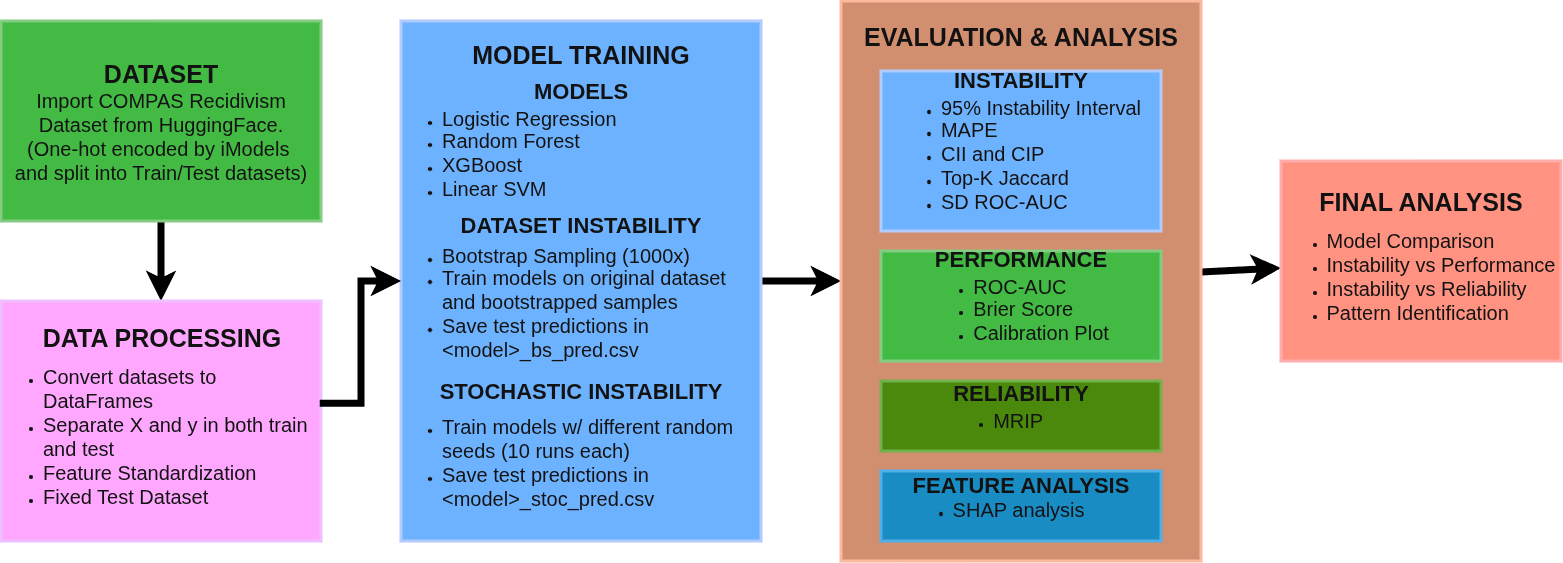
\includegraphics[width=1\textwidth]{proposed_methodology.png}
\caption{Overview of the proposed methodology for evaluating dataset and stochastic instability in ML models.}\label{fig:Proposed Methodology Implementation}
\end{figure}

\begin{enumerate}
  \item \textbf{Dataset Importing and Processing:}
  The dataset is imported using the \texttt{datasets} library from HuggingFace. Since the source already contains separate training and test datasets, the program imports each dataset into panda DataFrames where the test dataset is fixed throughout all experiments and the training dataset is used for repeated model training.\\

  Because the selected version of the COMPAS Recidivism Dataset has already been one-hot encoded and prepared for ML use, only minimal preprocessing is required, specifically Feature standardization using \texttt{StandardScaler}. The scaler is fit on the training data and subsequently applied to the test data using the same parameters to prevent data leakage. This preprocessing step is performed prior to model training and remains fixed across all bootstrap and stochastic iterations.\\

  Before performing repeated training procedures, each model is trained once on the original training dataset using a fixed random seed $s = 0$. The predictions generated from this baseline model serve as a reference for evaluating instability metrics.

  \item \textbf{Model Training For Dataset Instability:}
  To evaluate dataset instability, the study employs bootstrap resampling approach~\cite{efron2000bootstrap}, which is a sampling method that generates proxy datasets by repeatedly drawing samples with replacement from the original dataset. This allows the study to simulate how model predictions may change under different possible versions of the same dataset. Moreover, bootstrapped resampling was also used by Riley and Collins~\cite{riley2023stability} in their study. The same hyperparameters is held constant across all bootstrap iterations. \\

  A total of 1000 bootstrap samples is generated from the original training dataset using sampling with replacement. This number is selected to ensure a stable estimation of prediction variability across runs while maintaining computational feasibility. Each bootstrapped dataset maintains the same size as the original training set but contains slight variations in data composition due to the resampling process. These variations simulate realistic perturbations in the data, such as missing or duplicated observations. To ensure that dataset sources of instability are isolated from the stochastic sources, a fixed random seed $ s = 0 $ is implemented for all dataset instability experiments.\\ 

  Each model is then be retrained independently on every bootstrapped sample with a fixed random seed of $ s = 0$. After training, predictions is generated using the fixed test dataset and stored in structured CSV files with the filename $<model>\_bs\_pred.csv$, where each column represents the predicted scores from a specific training run. This organized storage enables direct comparison of predictions across multiple runs for each individual.\\

  By repeating this process across all bootstrapped samples, the study produces a distribution of predictions for each test instance which serves as the basis for computing instability metrics in later stages of the methodology.

  \item \textbf{Model Training For Stochastic Instability:}
  To evaluate stochastic instability, the models are trained multiple times with different random seeds while using the same fixed training dataset to ensure that the stochastic sources of instability are isolated from the dataset sources. The study follows a similar approach by Lopez-Martinez et al.~\cite{lopez2022instability}.\\

  Each model is trained for 10 independent runs using the predefined seed set $S = \{1,\dots,10\}$. Each seed controls all stochastic components of the model training process, ensuring that variability is solely attributable to stochastic effects.\\

  This variation in random seed introduces a controlled randomness into the training process, allowing the study to isolate the effects of stochasticity on model behavior. Despite using the same dataset and configuration, these stochastic factors may lead to differences in learned model parameters and, consequently, prediction outputs. It is noted, however, that stochastic variability may differ across models depending on their underlying training mechanisms. Models such as Random Forest and XGBoost incorporate inherent randomness during training, while models such as Logistic Regression and LinearSVC may exhibit limited stochastic variation under default deterministic settings.\\

  After each training run, predictions is generated using the fixed test dataset. This allows any observed differences in predictions to be attributed solely to stochastic variation rather than changes in the data. The predicted scores for each instance in the test dataset is recorded for every run. \\

  Similar to the dataset instability procedure, all predictions is stored in structured CSV files, where each column corresponds to a specific training run with a distinct random seed. This format enables direct comparison of predictions across runs at the individual level.\\

  By repeating this process across multiple random seeds, the study generates a distribution of predictions for each test instance under stochastic conditions. These distributions are then used in the later stages of the methodology.

  \item \textbf{Evaluating Model Instability, Performance, Fairness, and Reliability:}
  Following the repeated training procedures for both dataset and stochastic instability, the study evaluates each model using a combination of instability, performance, and reliability metrics for both dataset and stochastic instability.

  95\% Stability Intervals is constructed by computing the percentile range of predictions for each instance, providing a visual representation of the spread and uncertainty in predicted scores.

  To measure instability in predicted scores, the Mean Absolute Prediction Error (MAPE) is computed for each test instance across all runs. This quantifies the average variation in predicted risk scores, where higher values indicate greater instability. 

  To assess instability in classification outcomes, the Classification Instability Index (CII) is calculated. This metric measures how frequently an individual's predicted class label changes across different runs. Higher CII values indicate greater inconsistency in classification decisions, which is critical in applications such as RRP where classification outcomes directly influence decision-making. 

  The study also evaluates ranking instability using the Top-K Jaccard Similarity. For each run, the top K\% of individuals with the highest predicted risk scores is identified, and the overlap between these sets across runs is measured. Lower similarity values indicate greater inconsistency in identifying high-risk individuals.

  The Brier Score and ROC-AUC is computed for every run separately within each fold and evaluation set (Validation and Test). For each fold, the mean and sample standard deviation across that fold's runs is reported. For Brier Score, the within-fold SD describes run-to-run variability in probabilistic error; calibration is assessed from the reliability curves. Fold-level summaries remain separate; no overall mean or standard deviation across folds is calculated.

  In addition to instability, model performance is evaluated to ensure that stability is considered alongside predictive effectiveness. Higher within-fold run variability in ROC-AUC indicate instability in model performance. Moreover, calibration plots is generated separately for each fold to assess how well the predicted scores align with the observed outcomes. These plots compare predicted risk scores with actual recidivism frequencies, where a curve close to the diagonal indicates well-calibrated predictions. Deviations from this diagonal suggest overestimation or underestimation of risk. While primarily used as a visual diagnostic tool, calibration plots provide complementary insight into the reliability of probability estimates across different models and training conditions.

  The study also incorporates a fairness metric based on false positive rate (FPR) differences across groups to assess potential disparities in error behavior among different demographic groups. Specifically, the False Positive Rate (FPR) measures the proportion of individuals incorrectly classified as high risk among those who do not reoffend, and the difference in FPR between groups is used to quantify disparity in misclassification rates. This provides a group-level assessment of whether the model disproportionately produces false alarms for certain populations.

  Furthermore, the study incorporate a reliability metric to assess the trustworthiness of individual predictions. The Model Reliability for Individual Prediction (MRIP) is used to estimate the likelihood that a model's prediction error remains within an acceptable range for each instance. This provides a more granular evaluation of reliability compared to aggregate performance metrics.

  All computed metrics is summarized and compared across models and across both types of instability. These analyses enable the identification of patterns in instability behavior and provide a comprehensive assessment of how consistent, accurate, and reliable each model is under varying training conditions.

  \item \textbf{SHapley Additive exPlanations:}
  SHAP values is computed for the first validation defendant in each fold and for the first defendant in the fixed test set. The same test defendant is evaluated in every fold. For each selected case, SHAP is computed for every bootstrap run in the dataset-instability experiment and every random-seed run in the stochastic-instability experiment, for Logistic Regression (LR), LinearSVC (LSVC), XGBoost (XGB), Random Forest (RF), and MLP.\@

  The explainer and reference data vary by model. TreeExplainer is used for RF and XGB without a separate background dataset, so it uses its default tree-path-dependent reference based on training counts in tree leaves. LinearExplainer is used for LR with the run's training data as its reference data. For LSVC, shap.Explainer is given the model's predict\_proba function and the full training data. For MLP, KernelExplainer is given predict\_proba and a random sample of up to 50 training rows selected with random\_state=42; SHAP values are estimated using nsamples=10.

  The saved raw per-fold files contain the defendant ID, feature name, and one SHAP value column for each run. Post-analysis computes and saves the signed mean SHAP value across runs for each selected defendant, feature, and fold. It does not compute run-wise standard deviations, global mean absolute feature importance, or SHAP summary or variability plots; the analysis is therefore limited to the per-run values and their signed means.

  The explainers do not use a common output space. LR LinearExplainer values represent the logistic model's log-odds output, and the default raw XGB TreeExplainer values represent the positive-class raw margin (log odds). RF TreeExplainer values and the selected LSVC and MLP predict\_proba outputs represent the positive-class probability. SHAP magnitudes are consequently interpreted within each model and output scale, not compared directly across models.

  \item \textbf{Identifying Patterns and Relationships:}
  After computing instability, performance, fairness, reliability, and SHAP-based feature contribution metrics,  the study proceeds with the analysis.
  
  First, instability metrics is compared across all models to determine which models exhibit higher levels of dataset and stochastic instability. This includes examining differences in probability variability (MAPE and stability intervals), classification inconsistency (CII), and ranking instability (Top-K Jaccard Similarity). These comparisons allow the study to identify whether certain model types are more sensitive to data perturbations or stochastic factors.

  % After computing instability, performance, fairness, reliability, and SHAP-based feature contribution metrics, the study proceeds with analyzing patterns and relationships observed from the computed metrics to better understand how instability, specifically dataset and stochastic, manifests in different models.

  Following the analysis of each model's instability sensitivity to dataset and stochastic factors, the study contextualizes the instability metrics of its corresponding instability type with its respective computed performance, fairness, reliability, and feature contribution metrics. 

  Model instability is compared to performance metrics to identify relationships and patterns between them such as  whether instability may affect model performance and accuracy. 

  The study also examines the relationship between instability and fairness in terms of the FPR differences across demographic groups. This enables a group-level evaluation of whether the model generates disproportionately higher false positive predictions for specific demographics, providing a more nuanced perspective on fairness than what is captured by overall accuracy or other aggregate performance measures.

  The study also examines the relationship between instability and reliability by comparing instability metrics with MRIP values. This analysis helps determine whether increased prediction variability corresponds to lower reliability at the individual prediction level, which is critical in high-stakes applications such as RRP.\@

  Performance, fairness, and reliability metrics also provide context to model instability, identifying whether a model with either high or low instability is valid for RRP when considering its performance, fairness, and reliability metrics.

  SHAP outputs is reviewed for the selected validation and test defendants. The analysis examines the per-run signed feature contributions and their signed mean within each fold, interpreting them on the output scale used by each model. It does not treat these values as global feature-importance or variability summaries, and raw magnitudes are not compared directly across models.

  % the fuck is this lol edit it kay it's supposed to talk about the overal synthesis/explainability of the models
  Finally, the results from all analyses is synthesized to provide a comprehensive understanding of the overall instability of each model. 
\end{enumerate}
\newpage

\section{Preliminary Results}
Preliminary experiments were conducted to validate the experimental pipeline and ensure that the proposed evaluation framework produces stable and interpretable outputs. At this stage, results are available only for dataset instability with the models Logistic Regression, Random Forest, and XGBoost, while Linear SVM is still under implementation. \\

Initial outputs include instability visualizations (CII Plots), percentile-based variability summaries, and ROC curves. These results serve as a sanity check for the proposed methodology rather than final comparative conclusions across all models.

\begin{figure}[ht]
\centering
\begin{subfigure}{0.32\textwidth}
\centering
\includegraphics[width=\linewidth]{../src/metrics/Dataset/CII/LR/CII_LR_Dataset_Test_Fold_1.png}
\caption{Logistic Regression}
\end{subfigure}
\hfill
\begin{subfigure}{0.32\textwidth}
\centering
\includegraphics[width=\linewidth]{../src/metrics/Dataset/CII/RF/CII_RF_Dataset_Test_Fold_1.png}
\caption{Random Forest}
\end{subfigure}
\hfill
\begin{subfigure}{0.32\textwidth}
\centering
\includegraphics[width=\linewidth]{../src/metrics/Dataset/CII/XGB/CII_XGB_Dataset_Test_Fold_1.png}
\caption{XGBoost}
\end{subfigure}
\caption{Preliminary CII Distribution Graphs Across Models}
\end{figure}

Figure 2 presents a bard-based summary of CII values across models. This serves as an initial validation that the bootstrap-based sampling procedure produces observable variability in model predictions.

\begin{figure}[ht]
\centering
\includegraphics[width=\linewidth]{../src/metrics/Dataset/95_Prediction_Error/By_Evaluation/95_Prediction_Error_Dataset_Test_Across_Folds_Boxplot.png}
\caption{Preliminary 95\% Instability Percentile Across Models}
\end{figure}

Figure 3 summarizes the upper tail of prediction variability using the 95th percentile across runs. This is used as a preliminary indicator of the range of instability observed under repeated sampling. Based on the figure, differences in percentile distributions can be observed across the models.

\newpage
\begin{figure}[ht]
\centering
\begin{subfigure}{0.32\textwidth}
\centering
\includegraphics[width=\linewidth]{../src/metrics/Dataset/95_Prediction_Error/By_Evaluation/95_Prediction_Error_Dataset_Test_Across_Folds_Boxplot.png}
\caption{Logistic Regression}
\end{subfigure}
\hfill
\caption{Preliminary ROC Curve For Bootstrap Sample 20}
\end{figure}

Figure 4 shows the ROC curves of the evaluated models at bootstrap sample 20 under the current experimental setup. This is included as a preliminary check to verify that the models produce valid probabilistic outputs suitable for downstream evaluation. \\

\newpage
\section{Schedule of Activities}
\subsection{2026}

\begin{longtable}{
 >{\raggedright\arraybackslash}p{1.1cm}
 >{\raggedright\arraybackslash}p{2.5cm}
 >{\raggedright\arraybackslash}p{4cm}
 *{8}{>{\centering\arraybackslash}p{0.6cm}}
}
\caption{Schedule of Activities (2026)}\label{tab:schedule}\\
\toprule
\textbf{Objective} & \textbf{Target Activities} & \textbf{Target Accomplishments} & \multicolumn{8}{c}{\textbf{2026 (Months)}} \\
\cmidrule(lr){4-11}
& & & May & Jun & Jul & Aug & Sept & Oct & Nov & Dec \\
\midrule
\endfirsthead

\toprule
\textbf{Objective} & \textbf{Target Activities} & \textbf{Target Accomplishments} & \multicolumn{8}{c}{\textbf{2026 (Months)}} \\
\cmidrule(lr){4-11}
& & & May & Jun & Jul & Aug & Sept & Oct & Nov & Dec \\
\midrule
\endhead

Obj. 1
& Assess dataset instability by retraining models on bootstrapped, K-fold training samples.
&
(1) Generate K-fold splits from the training dataset, and generate bootstrapped samples from the split data, using the excluded split fold as the validation for each fold.\newline
(2) Train each model on the original fold, then on its bootstrapped samples.\newline
(3) Save the generated predictions from the fixed test and validation datasets in csv files separated by folds.
& \cellcolor{gray!30} & \cellcolor{gray!30} & \cellcolor{gray!30} & \cellcolor{gray!30} & & & & \\
\midrule

Obj. 2
& Assess stochastic instability by retraining models with different random seeds across K-fold training partitions.
&
(1) Generate K-fold splits from the training dataset and use the excluded split fold as the validation for each fold.\newline
(2) Train each model multiple times on the training data by fold using different random seeds using default model parameters.\newline
(3) Save the generated predictions from the fixed test and validation datasets in csv files separated by folds.
& \cellcolor{gray!30} & \cellcolor{gray!30} & \cellcolor{gray!30} & \cellcolor{gray!30} & & & & \\
\midrule

Obj. 3
& Evaluate instability, performance, fairness, reliability, and feature contributions using validation and official test predictions.
&
(1) Measure model instability using instability metrics.\newline
(2) Measure model predictive performance using performance metrics.\newline
(3) Measure model fairness using fairness metrics.\newline
(4) Measure model reliability using a reliability metric.\newline
(5) Save per-run SHAP contributions and their signed means for selected validation and test defendants. \newline
(6) Save all computed instability, performance, fairness, reliability, and feature contribution results and generated visualizations for analysis.
& & & \cellcolor{gray!30} & \cellcolor{gray!30} & \cellcolor{gray!30} & & & \\
\midrule

Obj. 4
& Analyze how instability, model structure, and feature contributions relate to predictive inconsistency.
&
(1) Compare results from instability metrics across all models to identify which models exhibit higher dataset and stochastic instability.\newline
(2) Compare results from performance, fairness, and reliability metrics to instability metrics to identify patterns and relationships.\newline
(3) Contextualize model viability using instability metrics with performance, fairness, and reliability metrics.\newline
(4) Review signed mean SHAP contributions for selected defendants within each model and fold.\newline
(5) Interpret SHAP contributions in light of each model's explained output scale.\newline
(6) Synthesize the results to explain overall model instability.
& & & & & \cellcolor{gray!30} & \cellcolor{gray!30} & \cellcolor{gray!30} & \cellcolor{gray!30} \\
\bottomrule

\end{longtable}

\bibliographystyle{unsrt}
\bibliography{references}

\end{document}
